\section{684 --- Redundant Connection}
In this problem, a tree is an \textbf{undirected} graph that is connected and has no cycles.

The given input is a graph that started as a tree with $N$ nodes (with distinct values $1, 2, \ldots, N$), with one additional edge added. The added edge has two different vertices chosen from 1 to $N$, and was not an edge that already existed.

The resulting graph is given as a 2D-array of edges. Each element of edges is a pair $[u, v]$ with $u < v$, that represents an undirected edge connecting nodes $u$ and $v$.

Return an edge that can be removed so that the resulting graph is a tree of $N$ nodes. If there are multiple answers, return the answer that occurs last in the given 2D-array. The answer edge $[u, v]$ should be in the same format, with $u < v$.

\paragraph{Example 1:}
\begin{flushleft}


\textbf{Input}: \lstinline[language=C++, basicstyle=\small\ttfamily, keywordstyle=\bfseries\color{green!40!black}]|[[1,2], [1,3], [2,3]]|

\textbf{Output}: \lstinline[language=C++, basicstyle=\small\ttfamily, keywordstyle=\bfseries\color{green!40!black}]|[2,3]|

\textbf{Explanation}: The given undirected graph will be like this:

\begin{figure}[H]
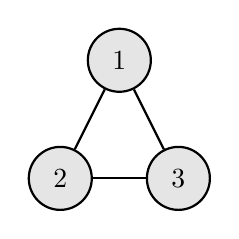
\begin{tikzpicture}
[every node/.style={draw, circle, fill=gray!20!, minimum size=8mm},
thick]
\node{1}
child{node(0){2}}
child{node(1){3}};
\draw (0)--(1);
\end{tikzpicture}
\end{figure}
\end{flushleft}

\paragraph{Example 2:}
\begin{flushleft}


\textbf{Input}: \lstinline[language=C++, basicstyle=\small\ttfamily, keywordstyle=\bfseries\color{green!40!black}]|[[1,2], [2,3], [3,4], [1,4], [1,5]]|

\textbf{Output}: \lstinline[language=C++, basicstyle=\small\ttfamily, keywordstyle=\bfseries\color{green!40!black}]|[1,4]|

\textbf{Explanation}: The given undirected graph will be like this:
\begin{figure}[H]
\begin{tikzpicture}
[every node/.style={draw, circle, fill=gray!20!, minimum size=5mm},
thick]
\node(0){5};
\node[right=8mm of 0](1){1};
\node[right=8mm of 1](2){2};
\node[below=8mm of 1](4){4};
\node[below=8mm of 2](3){3};
\draw (0) -- (1);
\draw (1) -- (2);
\draw (1) -- (4);
\draw (2) -- (3);
\draw (4) -- (3);
\end{tikzpicture}
\end{figure}
\end{flushleft}

\paragraph{Note:}
\begin{itemize}
\item The size of the input 2D-array will be between 3 and 1000.
\item Every integer represented in the 2D-array will be between 1 and $N$, where $N$ is the size of the input array.
\end{itemize}

\subsection{DFS}
题目的主要意图是在tree中检测出cycle。

We will detect cycle in the process of building adjacent list. For each edge $(u,v)$, we run a depth first search if there already exist a path from $u$ to $v$ before inserting $(u,v)$ into the adjacent list. Since this is a undirected graph, we don't need to search a path from $v$ to $u$.

The process of searching cycle is trivial: we first check if $v$ is already be a adjacent node of $u$. If it is not, we recursively deep into the adjacent nodes of $u$ to check. In this process, we must not consider the nodes we have already visited by adding current visit node number as the recursive function parameter.

\setcounter{lstlisting}{0}
\begin{lstlisting}[style=customc, caption={DFS}]
vector<int> findRedundantConnection( vector<vector<int>>& edges )
{
    vector<unordered_set<int>> adj( edges.size() + 1 );

    //build ajacent list
    for( const auto& edge : edges )
    {
        //if there is already a path
        //from edge[0] to edge[1]
        //there is a cycle
        if( dfs( edge[0], edge[1], adj, -1 ) )
        {
            return edge;
        }

        //since this is a undirected graph
        //we need to add both into their adjacent list
        adj[edge[0]].insert( edge[1] );
        adj[edge[1]].insert( edge[0] );
    }

    return {};
}

bool dfs( int start, int end, vector<unordered_set<int>>& G, int pre )
{
    //if end is the adjacent node of start
    //we found the path
    if( G[start].find( end ) != G[start].end() )
    {
        return true;
    }

    for( int next : G[start] )
    {
        //avoid visit
        //nodes that have been visited
        if( next == pre )
        {
            continue;
        }

        if( dfs( next, end, G, start ) )
        {
            return true;
        }
    }

    return false;
}
\end{lstlisting}

\subsection{Union Find}
For each edge $(u,v)$, we first find the parents of $u$ and $v$, say $p_u$ and $p_v$. If $p_u=p_v$, we know there already a path between $u$ and $v$ except direct edge $(u,v)$, i.e. a cycle. Otherwise, we set parent of $p_u$ to $p_v$ (set parent of $p_v$ to $p_u$ can also work).

\begin{lstlisting}[style=customc, caption={Union Find}]
vector<int> findRedundantConnection( vector<vector<int>>& edges )
{
    int N = static_cast<int>( edges.size() + 1 );

    vector<int> parents( N + 1, 0 );

    for( int i = 1; i <= N; ++i )
    {
        parents[i] = i;
    }

    for( const auto& edge : edges )
    {
        int p0 = find( parents, edge[0] );
        int p1 = find( parents, edge[1] );

        if( p0 == p1 )
        {
            //a path except current edge
            //exists between edge[0] and edge[1]
            //a cycle detected
            return edge;
        }

        //set parent of edge[0]
        //to parent of edge[1]
        parents[p0] = p1;
    }

    return {};
}

int find( vector<int>& parents, int x )
{
    while( x != parents[x] )
    {
        x = parents[x];
    }

    return x;
}
\end{lstlisting}